% This file was created by matlab2tikz.
%
%The latest updates can be retrieved from
%  http://www.mathworks.com/matlabcentral/fileexchange/22022-matlab2tikz-matlab2tikz
%where you can also make suggestions and rate matlab2tikz.
%
\definecolor{mycolor1}{rgb}{0.00000,0.44700,0.74100}%
\definecolor{mycolor2}{rgb}{0.85000,0.32500,0.09800}%
\definecolor{mycolor3}{rgb}{0.92900,0.69400,0.12500}%
\definecolor{mycolor4}{rgb}{0.49400,0.18400,0.55600}%
\definecolor{mycolor5}{rgb}{0.46600,0.67400,0.18800}%
%
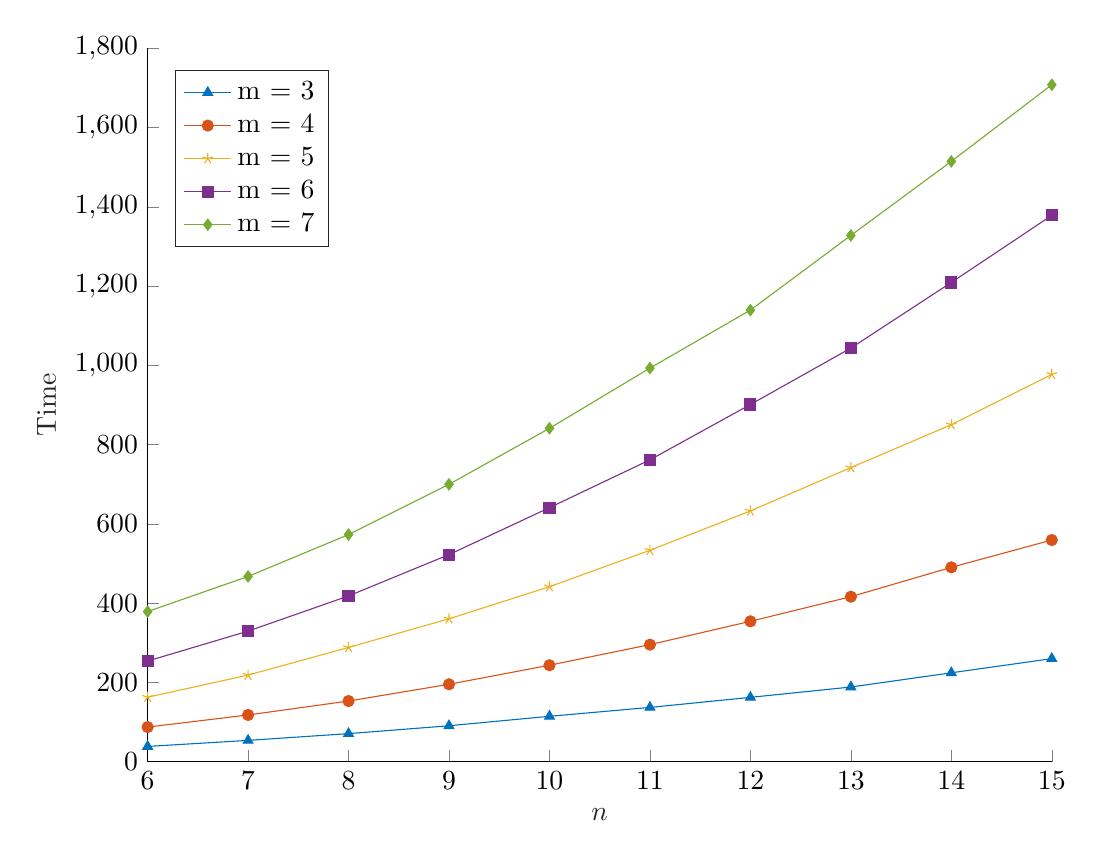
\begin{tikzpicture}

\begin{axis}[%
width=4.521in,
height=3.566in,
at={(0.758in,0.481in)},
scale only axis,
xmin=6,
xmax=15,
xlabel style={font=\color{white!15!black}},
xlabel={$n$},
ymin=0,
ymax=1800,
ylabel style={font=\color{white!15!black}},
ylabel={Time},
axis background/.style={fill=white},
title style={font=\bfseries},
%title={Average ticks until solution as a function of n. On n 	imes m grid. (k = 5)},
axis x line*=bottom,
axis y line*=left,
legend style={at={(0.03,0.97)}, anchor=north west, legend cell align=left, align=left, draw=white!15!black}
]
\addplot [color=mycolor1, mark=triangle*]
  table[row sep=crcr]{%
6	38.504\\
7	53.806\\
8	70.83\\
9	90.72\\
10	114.586\\
11	136.996\\
12	162.38\\
13	188.464\\
14	224.378\\
15	260.088\\
};
\addlegendentry{m = 3}

\addplot [color=mycolor2, mark=*]
  table[row sep=crcr]{%
6	87.4\\
7	117.924\\
8	153.106\\
9	195.388\\
10	243.508\\
11	295.416\\
12	354.272\\
13	416.438\\
14	490.564\\
15	559.456\\
};
\addlegendentry{m = 4}

\addplot [color=mycolor3, mark=star]
  table[row sep=crcr]{%
6	162.66\\
7	218.6\\
8	288.344\\
9	360.608\\
10	441.666\\
11	533.534\\
12	632.866\\
13	742.246\\
14	850.5\\
15	977.504\\
};
\addlegendentry{m = 5}

\addplot [color=mycolor4, mark=square*]
  table[row sep=crcr]{%
6	254.028\\
7	329.554\\
8	418.372\\
9	522.656\\
10	641.202\\
11	761.858\\
12	901.468\\
13	1043.858\\
14	1209.536\\
15	1378.886\\
};
\addlegendentry{m = 6}

\addplot [color=mycolor5, mark=diamond*]
  table[row sep=crcr]{%
6	378.886\\
7	467.542\\
8	573.198\\
9	700.01\\
10	841.392\\
11	993.348\\
12	1139.76\\
13	1328.168\\
14	1515.118\\
15	1708.482\\
};
\addlegendentry{m = 7}

\end{axis}
\end{tikzpicture}%